% =====================================================================
% Transfer boundaries in affective audio modelling
% Submission draft for IEEE Transactions on Affective Computing.
%
% This file replaces the bioRxiv/arXiv preprint version, archived at
% archive/main_preprint_2026-08.tex. The revision is not a reformatting:
% a pre-submission audit found that the preprint's organising claim --- that
% generalisation failures divide into two kinds with mutually exclusive
% remedies, one of which "cannot be bought back" --- is contradicted by this
% project's own measurements. reports/TAC_revision_audit.md records what
% changed, what was recomputed, and what was withdrawn. The short version:
%
%   * the few-shot learning curve the preprint attributed to same-domain
%     transfer was measured on cross-domain pairs, so the boundary the
%     preprint called unpurchasable is the one whose price it quoted;
%   * half of the environmental corpus is mixtures of thirty recordings, and
%     the cross-validation protocol did not group them, which inflated both
%     that corpus's ceiling and the apparent size of the domain gap;
%   * the "calibration, not sign" mechanism is contradicted by the
%     disaggregated intervention data and is in any case incompatible with a
%     rank-correlation metric;
%   * the stimulus-level reliability that set the physiological denominator is
%     reproduced by presentation position alone, so no fraction-of-ceiling can
%     be quoted on that boundary.
%
% What remains is a measurement paper rather than a framework paper, and the
% numbers in it are stronger for having lost the framework.
% =====================================================================
% =====================================================================
% Preamble --- IEEE Transactions on Affective Computing
%
% This replaces the single-column `article` layout used for the bioRxiv/arXiv
% preprint (kept at archive/preamble_preprint_2026-08.tex). IEEE Computer
% Society states without qualification that template use is mandatory for
% journal submissions, so the class, the bibliography style and the float
% handling are all fixed by the template rather than chosen:
%
%   https://www.computer.org/publications/author-resources
%     "Journals: Using an article template is required for journal submissions."
%   https://www.computer.org/csdl/journal/ta/write-for-us/15060
%     "Regular paper - 12 double column pages (Submissions may be up to 18
%      pages in length, subject to MOPC.)"
%
% Two page numbers therefore matter and are not the same thing. Twelve pages
% is the Mandatory Overlength Page Charge threshold ($220 for each page or
% fraction beyond it); EIGHTEEN is the hard cap on what may be submitted at
% all. The preprint ran to 40 single-column pages, which is roughly 25 in this
% layout, so the conversion is a compression job as much as a reformatting one:
% the long figure legends moved into the Supplementary Information, which TAC
% explicitly does not cap, and the Methods keep only what a reader needs to
% judge the result.
%
% Line numbering: the preprint carried a \iflinenums switch because arXiv puts
% submissions with margin line numbers on hold. IEEEtran has no such
% requirement and ScholarOne does not ask for them, so the switch is gone.
% =====================================================================
\documentclass[journal]{IEEEtran}

\usepackage[T1]{fontenc}
\usepackage[utf8]{inputenc}
\usepackage{microtype}

\usepackage{amsmath,amssymb}
\usepackage{graphicx}
\usepackage{booktabs}
\usepackage{multirow}
\usepackage{array}
\usepackage{url}
\usepackage[hidelinks]{hyperref}
\usepackage{xcolor}

% IEEEtran wants its own citation handling; cite.sty gives the sorted,
% compressed [3]--[5] form the journal uses.
\usepackage{cite}
\bibliographystyle{IEEEtran}

% Two-line table headers. Several tables have column headings far wider than
% the numbers beneath them, which in two columns runs the table past the
% measure; stacking the heading makes each column as wide as its data.
\newcommand{\thd}[2]{\begin{tabular}[b]{@{}c@{}}#1\\#2\end{tabular}}

\usepackage{upgreek}
\newcommand{\uV}{\ensuremath{\upmu\mathrm{V}}}

% ORCID iD as the linked green icon IEEE now sets after an author's name.
% Only J. Zhang has one; X. Yao does not, and an author without an ORCID simply
% carries no icon -- nothing is left blank and nothing is invented.
\usepackage{orcidlink}

% Shorthand for the two variants of the environmental corpus that the
% mixture-leakage control forces us to distinguish everywhere (Section
% III-C). Spelling them out each time costs a line per occurrence.
\newcommand{\emoAll}{Emo-Soundscapes (all 1{,}213)}
\newcommand{\emoOrig}{Emo-Soundscapes (600 originals)}

\hyphenation{op-tical net-works semi-conduc-tor}


\begin{document}

\title{Transfer Boundaries in Affective Audio Modelling:
Zero-Shot Loss, Measured Adaptation Cost, and the Limits of the
Available Evidence}

\author{Jingyi~Zhang\,\orcidlink{0009-0008-8738-3783} and Xiaotong~Yao%
\thanks{J. Zhang is with Shanghai Huangan Technology Co., Ltd., Shanghai,
China, and with Systems Neuroscience, Institute for Neuroscience, Department
of Health Sciences and Technology (D-HEST), ETH Zurich, Zurich, Switzerland
(e-mail: jingyi.zhang@hest.ethz.ch).}%
\thanks{X. Yao is with Shanghai Huangan Technology Co., Ltd., Shanghai,
China.}%
\thanks{The authors are engaged in the development of a commercial
sleep-audio product. See Section~\ref{sec:declarations}.}}

\markboth{IEEE Transactions on Affective Computing}%
{Zhang and Yao: Transfer Boundaries in Affective Audio Modelling}

\maketitle

\begin{abstract}
Affective audio models are usually evaluated inside the corpus they were
fitted on, and that optimism is rarely reported alongside the cost of removing
it. Using four rated-sound corpora, five representations and three
physiological corpora, we measure one mapping across four boundaries: to a new
corpus, to edited audio, to a sensor in place of self-report, and to an
individual listener. At each we report a within-corpus reference, what survives
unadapted, and what adaptation recovered. Within a corpus,
predicted arousal reaches 84\% of what annotation reliability permits. An
unadapted corpus swap costs about 15\% of that reference within the music
domain and 75\% across it; in both cases 100
target labels recover roughly half the gap, label-free second-moment alignment
recovers a quarter of the cross-domain gap, and four pretrained representations
recover little of it. Editing audio moves model output, not listeners, and
inconsistently across model and material. On the physiological boundary no
acoustic route exceeds a random-projection control, and no fraction-of-ceiling
is quotable: presentation position alone reproduces the target's reliability.
Per-person calibration loses to the population model at every budget existing
corpora supply. We separate what improved, what did not under the routes
tested, and what the evidence cannot decide.
\end{abstract}

\begin{IEEEkeywords}
Affective computing, cross-corpus generalisation, domain adaptation,
few-shot adaptation, soundscape emotion, annotator agreement,
personalisation, dataset bias.
\end{IEEEkeywords}

\IEEEpeerreviewmaketitle

% Applies the IEEEtran.bst control entry in references.bib. It has to come
% before the first real \cite, and it emits nothing.
\bstctlcite{IEEEtranBSTCTL:soundml}

% =====================================================================
\section{Introduction}

\IEEEPARstart{C}{hoosing} sound to shape affective state is an applied problem
with a growing evidence base and a well-known reporting convention: accuracy
is characterised within the collection on which the model was fitted. That
convention answers none of the questions an application asks. An application
changes the material, changes the \emph{kind} of material, changes how the
response is measured, and changes the listener. What matters is how much of
the mapping survives each of those changes and what it costs to recover what
is lost.

Both halves of that sentence are usually missing. Cross-corpus evaluations in
affective audio are typically reported zero-shot: a model is fitted on one
corpus, applied unchanged to another, and the resulting drop is reported as
the generalisation gap. A drop measured that way is an upper bound on the
problem, not an estimate of it, because no adaptation was attempted. The
complementary error is to report an adaptation method's gain without a control
that establishes how much of the gain is specific to the target rather than
generic to any distribution correction.

This paper measures both. We push one mapping --- group-averaged perceived
arousal from acoustic descriptors --- across four boundaries, ordered by how
far each moves from the fitting conditions: across corpora, across the
synthetic edits a deployed system applies to audio, across the level at which
the response is measured, and across individuals. At each boundary we report
three things: a within-corpus reference for that target, the fraction of it
that survives an unadapted crossing, and what each adaptation route we tested
recovered.

We separate three evidence states throughout, and label them explicitly rather
than collapsing them into a verdict:

\begin{enumerate}
\item \textbf{Improvement observed.} A named adaptation route recovered a
      quantified fraction of the gap.
\item \textbf{No improvement observed under the routes tested.} The routes we
      ran did not recover the gap. This bounds those routes; it does not bound
      every route, and it is not evidence that the information required is
      absent from the input.
\item \textbf{Insufficient evidence to determine cause or recoverability.} The
      design cannot separate the competing explanations, and we say which.
\end{enumerate}

This paper is a revision of a preprint \cite{zhang2026preprint} that reported
the same experiments under a stronger claim: that generalisation failures
divide into two kinds whose remedies are mutually exclusive, one of which no
quantity of data can repair. That claim does not survive its own evidence, for a reason worth
stating plainly because it is a general hazard. The learning curve that
priced the recoverable gap was computed on the cross-domain corpus pairs,
while the text attributed it to same-domain transfer and simultaneously
described the cross-domain boundary as unpurchasable. The figure legend was
correct and the prose was not. We report the corrected attribution here,
withdraw the framework it supported, and record the full audit in the
supplementary material.

Two findings of independent methodological value emerged from that audit, and
both concern corpora in wide use. Half of Emo-Soundscapes is mixtures of
thirty source recordings, and its distributed metadata gives every clip its
own group identifier, so the standard grouped cross-validation that authors
apply to it does not prevent near-duplicate clips from spanning folds
(Section~\ref{sec:hazards}). And in PMEmo, stimulus-level reliability of
electrodermal measures is reproduced --- in one case exceeded --- by
presentation position alone, so those measures cannot be used as a
stimulus-driven ceiling without a position control
(Section~\ref{sec:channel}). Anyone reusing either corpus is affected.

% =====================================================================
\section{Related Work}
\label{sec:related}

\subsection{Cross-corpus affective audio prediction}

That affective audio models degrade across corpora is established rather than
novel. In speech, cross-corpus emotion recognition has been surveyed and
benchmarked repeatedly, with normalisation strategies shown to account for a
substantial share of the nominal gap \cite{schuller2010crosscorpus,
zhang2019crosscorpus}. In music, cross-dataset evaluation reports similar
degradation and traces part of it to differences in annotation protocol rather
than in audio \cite{hu2017crossdataset}, and reviews note that most reported
accuracies are within-corpus \cite{yang2012machine, panda2023review}. Dataset
bias in audio, as in vision, makes corpus identity itself predictable
\cite{torralba2011unbiased}.

Our contribution is not the existence of the gap but its \emph{pricing}. Where
those studies report a zero-shot drop, we report the drop alongside what a
named budget of target-side labels and what a label-free alignment recover,
with a sham control that separates target-specific from generic gain. We also
add a boundary those studies do not cross: between two sound domains that
share no material, rather than between two corpora of the same kind.

\subsection{Unsupervised and few-shot domain adaptation}

Second-moment feature alignment (CORAL) \cite{sun2016coral} and subspace
alignment \cite{fernando2013subspace} are the two standard closed-form,
label-free baselines, and both are routinely reported without a control for
what the whitening step alone achieves. Few-shot target-side supervision is
the other standard route, and surveys of domain adaptation note that its
budget is rarely quoted in units an application can act on
\cite{wang2018deepda}. Work on affective audio specifically has applied
adversarial and discrepancy-based adaptation to cross-corpus speech emotion
\cite{abdelwahab2018domain}.

We add three things: the budget curve in labels rather than in epochs; a sham
alignment that establishes how much of CORAL's gain is target-specific; and a
decomposition of CORAL into per-dimension variance matching and correlation
structure matching, which turns out to locate most of the gain in the second.

\subsection{Personalisation and individual differences}

That listeners differ in how acoustic properties map onto their reported
affect is well documented, and personalised music emotion recognition has been
proposed repeatedly \cite{yang2007individuality, yang2009personalized, chen2014personalized}. The
question an application faces is narrower and less often asked: at what
observation count per person does a personal model beat the population model.
Work on the statistics of individual differences warns that between-person
variance components estimated from few observations per person are biased
upward \cite{rouder2019psychometrics}.

Our contribution is to estimate that break-even point on three corpora with a
common estimator and a per-cell null, and --- crucially --- to test it out of
sample. The out-of-sample test is the part that changes the conclusion: the
variance model places break-even at 67 to 318 observations per person, and a
direct held-out comparison returns a negative personalisation gain at every
budget the corpora actually supply.

\subsection{Annotator agreement as a ceiling}

Correcting an observed correlation for the unreliability of its target is
standard psychometrics \cite{spearman1904, nunnally1994}, and affective
computing has used inter-annotator agreement to bound achievable performance
\cite{grimm2007primitives}. Two errors are common and we guard against both:
dividing by the reliability rather than by its square root, which inflates the
corrected value by a factor of $1/\sqrt{r}$; and pairing a correlation
measured on one corpus with a reliability estimated on another.

We add the observation that a reliability estimate is only a ceiling if it is
stimulus-driven, and that this has to be tested. On the electrodermal measures
of PMEmo it fails: position alone reproduces the reliability, so no ceiling
can be quoted.

% =====================================================================
\section{Data and Methods}

\subsection{Corpora}

Four rating corpora were used: DEAM (music, $n = 1{,}233$)
\cite{aljanaki2017}, PMEmo (music, $n = 717$) \cite{zhang2018pmemo},
Soundtracks Set~1 (music, $n = 360$) \cite{eerola2011} and Emo-Soundscapes
(environmental, $n = 1{,}213$) \cite{fan2017emo}. ESC-50 \cite{piczak2015}
served as a second environmental corpus for the category control. The
prediction target throughout is group-averaged perceived arousal, rescaled to
$[-1, 1]$; the circumplex framing follows \cite{russell1980, eerola2013}.
Soundtracks additionally carries seven scales (valence, tension, anger, fear,
happiness, sadness, tenderness) on nine-point Likert scales, linearly
rescaled --- a monotone transformation that leaves all reported rank
statistics unchanged.

Soundtracks was included to test whether within-music transfer reflects shared
acoustic structure or a shared annotation tradition: it originates from a
different laboratory and decade, uses a categorical rather than continuous
protocol, and was assembled as a balanced design of twelve target emotions
$\times$ 30 excerpts.

One asymmetry between the music and environmental corpora must be recorded
here because it limits every cross-domain statement in this paper.
Emo-Soundscapes was annotated by \emph{pairwise comparison} and its ratings
derive from a ranking procedure, whereas the three music corpora were rated
directly on continuous or Likert scales. The corpora therefore differ in
annotation method as well as in sound domain, and with one environmental
corpus available the two cannot be separated (Section~\ref{sec:threats}).

\subsection{Audio preparation and descriptors}

All audio was resampled to 22{,}050\,Hz, centre-cropped to at most 30\,s, and
loudness-normalised to $-23$\,LUFS (ITU-R BS.1770) before any descriptor was
computed. Normalisation is not cosmetic: without it, corpus-specific mastering
levels act as an identifier that inflates apparent cross-corpus transfer
(Supplementary Fig.~S1). For the duration control, music excerpts were
additionally cropped to a 6\,s centred window to match the environmental
corpus.

\emph{Spectro-temporal (122).} Mel-frequency cepstral coefficients, spectral
centroid, bandwidth, contrast, flatness and roll-off, zero-crossing rate,
root-mean-square level, onset strength and onset rate, spectral slope, and
band-energy ratios. Each frame-level series is summarised by mean, standard
deviation, 10th, 50th and 90th percentiles, and the mean absolute first
difference, the last of which indexes rate of change rather than level.
Computed with librosa \cite{mcfee2015}.

\emph{Tonal (39).} A key-invariant chroma profile obtained by estimating the
tonic through correlation with Krumhansl--Kessler profiles
\cite{krumhansl1982} and rotating so the tonic occupies index~0; major- and
minor-key strength and their difference (mode score); chroma flux and entropy;
tonal centroids; an interval-consonance measure; sensory roughness after Plomp
and Levelt \cite{plomp1965}; and fundamental-frequency statistics. The full
list is in Supplementary Section~S11. Rotation to the tonic is essential
rather than convenient: an unrotated chroma vector encodes which key a piece
is in, which is arbitrary with respect to affect, so an unrotated
representation would let a model learn a corpus's key distribution. The
consonance weights are fixed a priori and are not fitted.

\emph{Pretrained representations.} Four families spanning four pretraining
paradigms were extracted over all four corpora: AST, supervised
classification on AudioSet \cite{gong2021ast, gemmeke2017audioset}; MERT,
self-supervised on music \cite{li2024mert}; Wav2Vec2, trained on speech
\cite{baevski2020wav2vec2}; and CLAP, audio--text contrastive learning
\cite{wu2023clap}. CLAP's pretraining set includes Freesound, from which
Emo-Soundscapes was built. We have not performed a sample-level overlap check
and therefore describe the overlap as \emph{possible at the corpus level}
rather than verified, and report CLAP separately throughout. The Wav2Vec2
checkpoint used is a speech model; we do not claim it is purely
self-supervised, only that its pretraining domain is speech.

\subsection{Models and evaluation}

Six regressors --- ElasticNet, support vector regression, $k$-nearest
neighbours, random forest, gradient boosting and XGBoost \cite{chen2016xgboost}
--- were evaluated by five-fold \texttt{GroupKFold} cross-validation.
Cross-corpus transfer fits on the whole of one corpus and evaluates on the
whole of another, with nothing refitted. Reported values are Spearman rank
correlations. Where a single value is reported for a cell it is the median over
the six algorithms unless stated otherwise; the preprint reported the best of
six in several places, which carries a winner's bias, and we now report the
best only where the quantity is explicitly an upper bound. Where a comparison
between conditions is made, all six are retained as paired observations and
the comparison is tested by Wilcoxon signed-rank.

\emph{Annotation reliability.} Per-rater judgements were split at random into
two halves, stimulus means computed within each, correlated, and corrected by
the Spearman--Brown formula \cite{spearman1904}; the reported value is the mean
over 200 random splits. Where a model's performance is expressed as a fraction
of what the annotation permits, the divisor is $\sqrt{r}$, not $r$: the
maximum correlation an errorless predictor can achieve against a target of
reliability $r$ is $\sqrt{r}$ \cite{nunnally1994}. Dividing by $r$ would
inflate the figure by $1/\sqrt{r}$.

\subsection{Two corpus-level hazards found during this revision}
\label{sec:hazards}

\subsubsection{Emo-Soundscapes contains mixtures of a small source set}

Of the 1{,}213 Emo-Soundscapes clips, 600 are single Freesound recordings and
613 are mixtures. The mixtures are built from five selected clips in each of
the six Schafer categories --- \textbf{thirty source recordings in total} ---
combined two or three at a time at two relative levels each. The distributed
filenames encode the constituents, from which we recover that the 613 mixtures
occupy only \textbf{161 distinct constituent sets}, a mean of 3.81 clips per
set and up to 8. Clips in one set differ only in mixing level.

The label table gives every clip its own group identifier, so
\texttt{GroupKFold} on this corpus is arithmetically identical to
\texttt{KFold}: near-duplicate mixtures span folds, and a training clip can be
a constituent of a test mixture. The protocol we and others describe as
preventing recording-level leakage does not prevent it here.

We therefore report every Emo-Soundscapes quantity twice: on all 1{,}213 clips
(\emph{published}, for comparability with prior work including our own
preprint) and on the 600 originals alone (\emph{clean}), where every clip is a
distinct recording and construction leakage is impossible. The effect is
substantial in both directions and is given in Table~\ref{tab:hazard}: the
within-corpus reference falls from 0.744 to 0.646, and median cross-domain
transfer \emph{rises} from 0.043 to 0.129, because a test set half composed of
near-duplicates distorts the ranking the metric is computed on. Both changes
shrink the apparent domain gap. The clean variant is the one we interpret.

\begin{table}[!t]
\centering
\caption{Effect of excluding the 613 Emo-Soundscapes mixture clips. Medians
over six algorithms; transfer medians over the six ordered corpus pairs of
each kind $\times$ six algorithms. Loss is per pair against the target
corpus's own within-corpus reference, then median over pairs.}
\label{tab:hazard}
\small
\setlength{\tabcolsep}{4pt}
\begin{tabular}{lcc}
\toprule
Quantity & \thd{All}{1{,}213} & \thd{600}{originals} \\
\midrule
Within-corpus $\rho$                 & 0.744 & 0.646 \\
Cross-domain $\rho$, median          & 0.043 & 0.129 \\
Cross-domain $\rho$, mean (s.d.)     & 0.058 (0.16) & 0.115 (0.15) \\
Cross-domain loss                    & 93.3\% & 74.9\% \\
Same-domain loss                     & 15.0\% & 15.0\% \\
\bottomrule
\end{tabular}
\end{table}

\subsubsection{PMEmo electrodermal reliability is reproduced by presentation
position}

Stimulus-level reliability of the three PMEmo electrodermal measures is 0.116
(skin-conductance response rate), 0.237 (phasic mean) and 0.234
(skin-conductance level slope). A sham that uses \emph{presentation position
alone} as the stimulus identifier returns 0.290, 0.283 and 0.267 --- that is,
249\%, 120\% and 114\% of the values obtained with the true stimulus labels.
The assignment of songs to positions in this corpus is itself significantly
non-random (intraclass correlation 0.041, $p = 0.005$), and regressing
position out of the measures reduces their reliability to 0.038, 0.081 and
0.206.

The consequence is not that the electrodermal measures are meaningless but
that their stimulus-level reliability is not established as stimulus-driven,
so it cannot serve as a ceiling. The preprint expressed the
cross-response-channel result as a percentage of exactly that ceiling. That
percentage is withdrawn (Section~\ref{sec:channel}).

\subsection{Adaptation routes}

Four label-free routes and one supervised route were compared, expressed as
the fraction of the gap between zero-shot transfer and a model trained on the
target corpus itself. Label-free: per-corpus $z$-scoring; CORAL
\cite{sun2016coral}, matching second moments in closed form; diagonal CORAL,
matching per-dimension variance only; and subspace alignment
\cite{fernando2013subspace}. Supervised: \emph{few-shot}, adding $k \in
\{10, 25, 50, 100, 200\}$ randomly chosen target-corpus examples to the
training set and evaluating on the remaining target examples, averaged over 20
resamples. The estimator for all adaptation results is ridge regression with a
cross-validated penalty, chosen on training data only.

Two reporting points follow from the audit. First, the few-shot numerator is
ridge while the denominator in the preprint was a six-algorithm median; we now
give both denominators. Second, $k = 200$ is unavailable for Soundtracks
($n = 360$, which the protocol's $k < n/2$ rule excludes), so the pair set at
$k = 200$ differs from the pair set at smaller $k$. We therefore report the
curve both over all available pairs and over the pairs present at every $k$.

\emph{Sham alignment.} CORAL performs two operations at once: it whitens the
source and it recolours towards the target. To separate them, the source was
also aligned to an unrelated third corpus, which by construction carries no
target-specific information. With a single environmental corpus this control
is only valid on half the pairs: when the source is environmental, the third
corpus is necessarily music and therefore in the \emph{target's} domain. We
report the sham separately for the three valid and three invalid pairs. The
preprint pooled them, which inverted the conclusion.

\subsection{Physiological corpora and controls}

\emph{EEG.} OpenNeuro ds002721 \cite{daly2018data}: 31 listeners, 19 scalp
channels at 1\,kHz referenced to FCz, six runs each, four containing ten 12\,s
music excerpts. Its stimuli are drawn from the same
published stimulus set as our fourth music corpus: the dataset's README gives
their source as \cite{eerola2011}, from which Soundtracks Set~1 also comes.
The two are therefore not independent material, and we have not been able to
establish from the distributed metadata which 40 of those excerpts were used. Event annotation follows BIDS and its EEG extension
\cite{gorgolewski2016, pernet2019}. Processing used MNE-Python
\cite{gramfort2013}: 50\,Hz notch, 1--45\,Hz bandpass, resampling to 250\,Hz.
Spectral and asymmetry measures were computed after average re-referencing;
coherence was computed on the recording reference, because average referencing
introduces a common component that inflates coherence.

Trial-wise measures (156): relative band power in five bands $\times$ five
regions as change from a 2\,s pre-onset baseline to a 1--14\,s window (26);
magnitude-squared coherence between all ten region pairs in five bands (50);
the imaginary part of coherency for the same pairs and bands (50),
insensitive to zero-lag volume conduction; and log-ratio asymmetry for six
homologous electrode pairs in five bands (30). Coherence and asymmetry are
included because the original analysis of these recordings located its effect
there \cite{daly2014}; restricting the set to band power would test the
conclusion on a representation that excludes the effect in question.

Four dataset-level controls were run before any substantive analysis, with the
rule that failure of any one halts interpretation: event bookkeeping; occipital
$>$ frontal relative alpha at rest; event-to-sample alignment via
independently annotated blink events; and a stimulus-locked evoked response
against a subject-wise sign-flip null with max-statistic correction
\cite{maris2007}. An individual-level control required each listener's EEG to
predict trial index, which is necessarily predictable given impedance and
vigilance drift. Multiplicity was controlled by Benjamini--Hochberg
\cite{benjamini1995}.

\emph{Electrodermal.} The PMEmo corpus carries song-level electrodermal
recordings, which we use for the acoustics-to-physiology comparison. This
pipeline was not described in the preprint and was not positive-controlled;
both are corrected here. Processing used NeuroKit2 \cite{makowski2021}
following standard recommendations \cite{boucsein2012}, with phasic--tonic
decomposition. Because no positive control for this pipeline passed --- and
because of the position confound above --- results from it are reported as
raw correlations against an explicit random-projection reference, and not as a
fraction of any ceiling.

A second electrodermal corpus, BIRAFFE2 \cite{kutt2022}, was analysed and
withdrawn: group-level habituation ran opposite to the established direction,
post-stimulus windows did not exceed random windows, and applied per
participant, none of 94 passed both controls (Supplementary Section~S2). It
supports no conclusion in this paper, including by way of corroboration.

\emph{Measured design requirement.} OpenNeuro ds003690
\cite{ds003690, ribeiro2019erp, ribeiro2019cardiac}: 75 adults (36 aged
19--30, 39 aged 50--70), 64-channel EEG, bipolar electrocardiogram and
binocular pupillometry at 500\,Hz during cued reaction-time tasks. Auditory
cues were 250\,ms pure tones at approximately 67\,dB(A); each participant
contributed 240 cues across two active tasks and 30 in a passive block. One
response measure was fixed per channel before analysis --- a fronto-central
window mean for EEG, a heart-rate change and a pupil-diameter change, each
against its own pre-cue baseline; exact windows and rejection criteria are in
Supplementary Section~S11. Each real cue was paired with a randomly placed
anchor in the same recording and all analyses operate on the difference, under
which sign-flipping is exact. Detection was assessed per participant with
5{,}000 sign flips at $\alpha = 0.05$ with Benjamini--Hochberg correction.

\subsection{Per-person calibration}

For each descriptor--outcome cell the between-person standard deviation
$\tau$ of the acoustic slope was estimated by restricted maximum likelihood
and compared with a null built by parametric bootstrap from that cell's own
design, because $\tau$ estimated from few observations per person is biased
upward: at 18 observations per person the estimator returns 0.11 when the true
value is zero. Break-even $n^{*}$ is the number of observations per person at
which the corrected spread exceeds the error in estimating it.

$n^{*}$ is a property of a variance model, not a demonstration that
personalisation pays. We therefore also report the direct test, which the
preprint omitted: fitting each listener their own slope and comparing
out-of-sample prediction against the population slope, at budgets
$n \in \{18, 30, 50, 100\}$.

Three settings were used, and they differ in more than the quantity under
study. Urban soundscape ratings come from ARAUS
\cite{ooi2024araus, ooi2025corrigendum} with
ISO-532 psychoacoustic descriptors (loudness, sharpness, roughness,
fluctuation strength) against the pleasantness and eventfulness axes; music
ratings come from DEAM with five spectro-temporal and tonal descriptors
against arousal and valence; and electrodermal responses come from PMEmo with
the same five descriptors against three electrodermal measures. Corpus,
descriptor set and outcome axis vary together across the three settings, so
differences between them cannot be attributed to any one of the three
(Section~\ref{sec:threats}).

\subsection{On claims of prior specification}

The preprint described several criteria as fixed in advance, pre-declared, or
falsifiable in advance. We have been unable to produce a traceable artifact
predating the corresponding analyses for any of them: the manuscript directory
was untracked in version control, the repository head predates most of the
runs, and only 2 of 199 run records carry a declared hypothesis. Those
phrasings are removed throughout and no analysis in this paper is presented as
preregistered. Where a criterion genuinely constrained a decision we say what
the criterion was and leave the reader to weight it accordingly.

% =====================================================================
\section{Results}

\subsection{Within-corpus reference and the annotation ceiling}

Across the four corpora, models predicting group-averaged perceived arousal
from 122 spectro-temporal descriptors reach Spearman $\rho = 0.65$--$0.81$
under grouped five-fold cross-validation (medians over six algorithms: DEAM
0.724, PMEmo 0.801, Soundtracks 0.810, \emoOrig{} 0.646).

Converting that into a distance from what the annotation permits requires the
model performance and the annotation reliability to come from the same
excerpts. On the 717 PMEmo excerpts, with the same descriptors, the same folds
and a per-rater split-half reliability of 0.935, the best of the six
algorithms reaches $\rho = 0.817$. Dividing by $\sqrt{0.935}$ puts it at
\textbf{84.4\%} (95\% CI 81.5--87.0\%) of the correlation an errorless
predictor of these annotations could attain.

Three qualifications belong with that figure, because it is optimistic in
three separate ways. It is the best of six algorithms evaluated on one set of
out-of-fold predictions, and the selection is not itself cross-validated. The
bootstrap resamples excerpts but does not refit, so it expresses sampling
variability in the evaluation and not in the fitting. And the reliability
estimate is carried through as fixed rather than as a quantity with its own
interval. The value should be read as an upper bound.

It should also not be read as a share of variance: the attenuation-corrected
value is a ratio of correlations, and squaring it puts the models at about
71\% of the reproducible variance, leaving roughly 29\% that better annotation
would not explain away. What the figure establishes is narrow and sufficient:
within a corpus, the remaining headroom for a better model is small relative
to the losses measured below.

Two framing choices affect the reference rather than the model. Treating
arousal as continuous rather than as a high-versus-low contrast retains the
middle of the range, which a median split discards along with a third to a
half of the excerpts (Supplementary Fig.~S2). And an additive glass-box model,
whose per-descriptor shape functions can be read directly, costs almost
nothing in accuracy relative to the tree ensembles (Supplementary Figs.~S3,
S4).

\subsection{Boundary 1: cross-corpus}
\label{sec:corpus}

\subsubsection{What an unadapted swap costs}

Transfer between corpora of the same domain is largely preserved. Over the six
ordered music-to-music pairs, each evaluated with the six algorithms (36
values in total, from 6 pairs --- the preprint described these as 36 pairs,
which overstated the number of independent units six-fold), transfer averages
$\rho = 0.591$ (s.d.\ 0.131). Expressed per pair against the target corpus's
own within-corpus reference, the median loss is \textbf{15.0\%} (range
10.7--35.6\%).

Between music and environmental sound, over the six ordered cross-domain pairs
$\times$ six algorithms, transfer averages $\rho = 0.115$ (s.d.\ 0.153) on the
clean environmental corpus, a median per-pair loss of \textbf{74.9\%} (range
58.6--115.6\%). On the published corpus the same quantities are 0.058 and
93.3\%; the difference is the mixture leakage of
Section~\ref{sec:hazards}, and it accounts for roughly two-thirds of the gap
between "four-fifths of performance lost" and "all of it"
(Fig.~\ref{fig:wall}).

\begin{figure*}[!t]
\centering
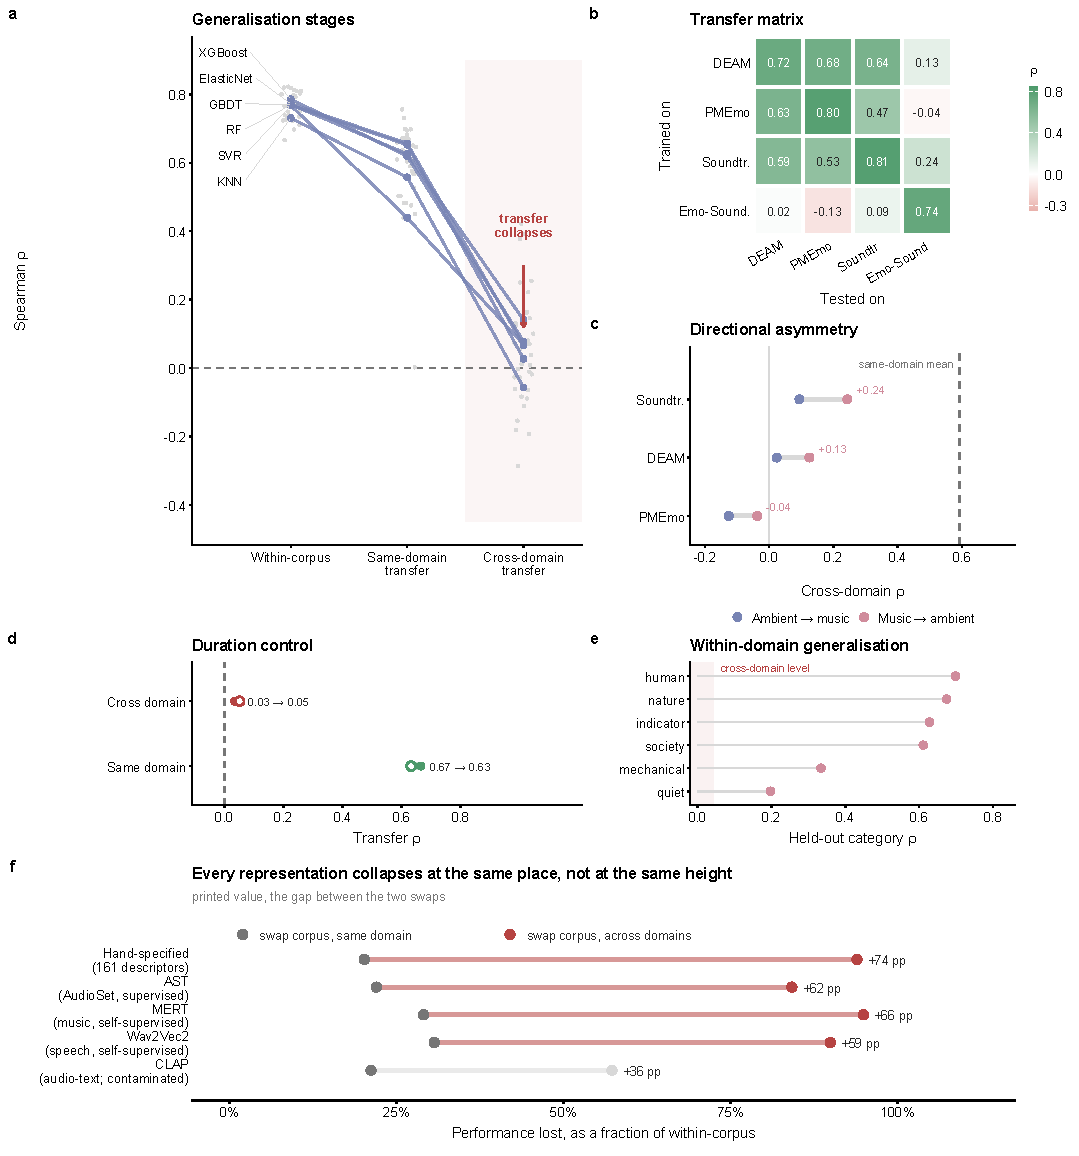
\includegraphics[width=\textwidth]{../reports/figures_r/Fig1_wall.pdf}
\caption{Arousal models transfer between corpora of the same sound domain far
better than across it, under every representation tested.
\textbf{(a)} Generalisation stages for six algorithms over 122
spectro-temporal descriptors, from within-corpus cross-validation through
same-domain transfer to cross-domain transfer; grey points are the individual
corpus pairs. \textbf{(b)} Transfer matrix averaged over algorithms; the
diagonal is within-corpus cross-validation. \textbf{(c)} The barrier is
asymmetric: inward transfer from the environmental corpus is uniformly low
($\rho \le 0.09$) while outward transfer is graded with the source corpus.
\textbf{(d)} Duration control (30\,s filled, 6\,s open). \textbf{(e)}
Leave-one-category-out generalisation within the environmental corpus.
\textbf{(f)} The same corpus swap costed under five representations, as the
fraction of each representation's own within-corpus performance lost. Values
in \textbf{(a)}--\textbf{(f)} are on the published environmental corpus, for
comparability with prior work; Table~\ref{tab:hazard} gives the leak-free
counterparts. Metric is Spearman $\rho$; all audio loudness-normalised to
$-23$\,LUFS. Extended description and source data in the Supplementary
Information.}
\label{fig:wall}
\end{figure*}

Three controls exclude the obvious confounds. Truncating music excerpts from
30\,s to a 6\,s window, matching the environmental corpus, leaves same-domain
transfer at 0.63 and cross-domain transfer near zero. Holding out each of the
six Schafer categories in turn leaves generalisation within the environmental
corpus at $\rho = 0.52$, so the collapse is not simply a response to unseen
content. Loudness normalisation before feature extraction removes a corpus
fingerprint that otherwise inflates apparent transfer (Supplementary
Fig.~S1).

The barrier is not symmetric. Transfer from the environmental corpus into each
of the three music corpora is uniformly low ($\rho \le 0.09$), while transfer
outward is graded: $-0.04$ from PMEmo, $+0.13$ from DEAM, $+0.24$ from
Soundtracks. Film soundtracks contain substantial atmospheric material, which
is a plausible account of that ordering but not one we measured; we report the
asymmetry and not an explanation for it.

\subsubsection{What adaptation recovers}

Calling a loss recoverable is only meaningful if the budget is quoted.
Fig.~\ref{fig:price} gives the recovery curves, and
Table~\ref{tab:adaptation} the numbers.

\begin{figure*}[!t]
\centering
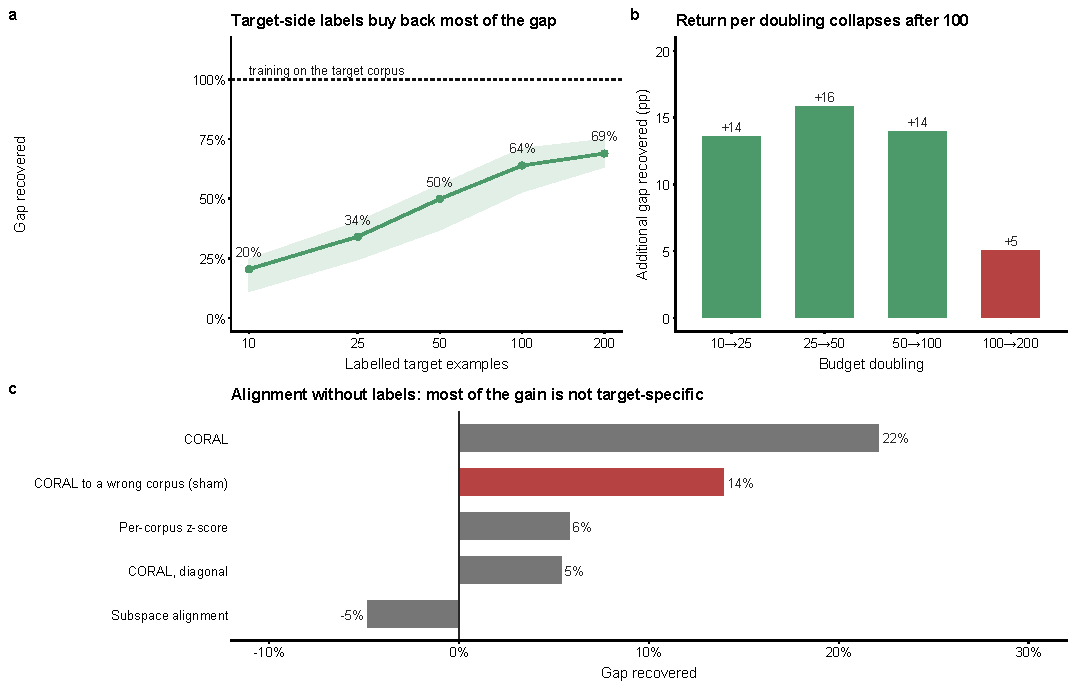
\includegraphics[width=\textwidth]{../reports/figures_r/Fig2_price.pdf}
\caption{What adaptation recovers on the corpus boundary, as the fraction of
the gap between zero-shot transfer and a model trained on the target corpus
itself. Environmental corpus without its mixture clips throughout.
\textbf{(a)} Budget curves for both kinds of corpus swap; line and points,
median over the six ordered pairs of each kind; band, interquartile range.
\emph{The preprint drew only the cross-domain curve and reported it as the
same-domain price.} \textbf{(b)} Label-free alignment with its sham control
split by validity: with one environmental corpus the ``unrelated third
corpus'' lies inside the target's own domain on three of the six pairs, and
the entire pooled sham effect comes from those three. \textbf{(c)} CORAL
decomposed; matching correlation structure, which is target-specific by
construction, contributes 80\% of the gain. Ridge estimator; metric is
Spearman $\rho$.}
\label{fig:price}
\end{figure*}

Target-side labels recover a substantial fraction of both gaps.
On the cross-domain pairs, 100 labels recover 57\% of the gap and 200 recover
71\%; on the same-domain pairs, 100 recover 50\% and 200 recover 77\%. The
two curves differ in shape rather than in whether a price exists: the
cross-domain curve rises faster at small budgets, because its zero-shot
starting point is much lower, while the same-domain curve overtakes it at 200.
Restricting both to the pairs present at every budget changes the cross-domain
values by at most 2 points and the same-domain values by up to 5, and does not
change the ordering.

\textbf{This is the correction that matters most in this revision.} The
preprint reported the cross-domain curve --- 20/34/50/64/69\% at
$k = 10/25/50/100/200$ --- and attributed it in the abstract and discussion to
transfer "to a new corpus of the same kind", while describing the cross-domain
boundary as one on which no purchase could be found. Both halves were wrong.
The curve is the cross-domain curve, so the boundary the preprint called
unpurchasable is precisely the one whose price it quoted; and the same-domain
price, which the preprint's numbers were said to describe, is different.

A label-free route also works. Correlation alignment recovers \textbf{25\%} of
the cross-domain gap with no target labels at all. The preprint discounted
this to roughly a third of its face value on the strength of a sham control
that appeared to recover 14\%. That pooled figure is an average over three
pairs where the sham is a valid negative control and three where it is not:
when the source corpus is environmental, the "unrelated third corpus" is
necessarily music and therefore in the target's domain. Separated, the valid
sham recovers $-11\%$ and the invalid sham $+25\%$. The entire apparent sham
effect comes from the invalid half, and CORAL's gain is therefore
\emph{more} target-specific than the preprint claimed, not less.
Decomposing CORAL confirms this: matching per-dimension variance alone
recovers 5\%, and the further 20 points --- 80\% of the total --- come from
matching correlation structure, which is target-specific by construction.
Subspace alignment is worse than doing nothing ($-5\%$).

\begin{table}[!t]
\centering
\caption{Adaptation on the corpus boundary, as the fraction of the gap between
zero-shot transfer and a model trained on the target corpus itself. Ridge
estimator, clean environmental corpus, median over the six ordered pairs of
each kind. Two denominators are given for the few-shot rows because the
numerator is ridge while the six-algorithm median is the reference used
elsewhere in this paper.}
\label{tab:adaptation}
\small
\setlength{\tabcolsep}{4pt}
\begin{tabular}{lcccc}
\toprule
& \multicolumn{2}{c}{Same domain} & \multicolumn{2}{c}{Across domains} \\
\cmidrule(lr){2-3}\cmidrule(lr){4-5}
Route & \thd{6-algo}{ref.} & \thd{ridge}{ref.} & \thd{6-algo}{ref.} & \thd{ridge}{ref.} \\
\midrule
10 target labels    & 8.6\%  & 7.5\%  & 18.8\% & 17.9\% \\
25 target labels    & 16.0\% & 13.7\% & 30.9\% & 28.7\% \\
50 target labels    & 33.9\% & 28.1\% & 43.5\% & 41.3\% \\
100 target labels   & 49.9\% & 43.6\% & 56.9\% & 54.3\% \\
200 target labels   & 76.5\% & 60.6\% & 71.0\% & 65.3\% \\
\midrule
CORAL (no labels)         & --- & --- & 25.0\% & --- \\
\quad diagonal only       & --- & --- & 4.9\%  & --- \\
\quad sham, valid pairs   & --- & --- & $-11.1$\% & --- \\
\quad sham, invalid pairs & --- & --- & 25.1\% & --- \\
Subspace alignment        & --- & --- & $-5$\% & --- \\
\bottomrule
\end{tabular}
\end{table}

One claim the preprint made about these curves does not survive either. It
reported that the return per doubling of the budget collapses after 100
labels, from a constant 14--16 points to 5. On the clean environmental corpus
the increments are 10, 14, 10 and 14 points --- no collapse, and the largest
increment is the last. The reported collapse was produced jointly by the
mixture leakage and by the change of pair set at $k = 200$. We therefore make
no claim about where the curve saturates: it had not saturated at the largest
budget we tested.

\subsubsection{Representation choice}

The most direct objection to the preceding is that 122 hand-specified
descriptors are too weak and that a representation learnt from a large audio
corpus would cross what they cannot. We extracted four pretrained
representations spanning four pretraining paradigms and repeated the transfer
analysis unchanged (Table~\ref{tab:families}).

The representations transfer between corpora and they do not cross between
domains. For a given representation, the same operation --- swap the corpus,
refit nothing --- costs 18--23\% of within-corpus performance when the new
corpus is in the same domain and 79--108\% when it is not. That disposes of
the alternative reading in which the embeddings simply fail to move between
datasets at all.

AST is the case that matters most, because AudioSet contains large numbers of
environmental categories and it is therefore the family that most ought to
cross. Here the mixture-leakage correction changes the conclusion
quantitatively. On the published environmental corpus, AST raises cross-domain
transfer from the hand-specified descriptors' $\rho = 0.047$ to $0.125$, a
factor of 2.7 --- the figure the preprint reported. On the leak-free corpus
the same comparison is $0.129$ against $0.162$: a difference of $+0.034$ and a
factor of \textbf{1.26}. Most of the apparent advantage of a large pretrained
representation over 122 hand-specified descriptors at this boundary was an
artifact of evaluating on a test set half composed of near-duplicate mixtures.
What remains is a small improvement in the expected direction.

Wav2Vec2, pretrained on speech, transfers across domains at $\rho = -0.034$ on
the leak-free corpus, which is to say not at all. MERT, pretrained on music,
reaches 0.085.

CLAP is the exception at a loss of 56\%, and it is the family whose
pretraining set includes the repository from which the environmental corpus
was built. It is not a generally stronger representation: within a corpus it
reaches 0.774 against AST's 0.770, and on music-to-music transfer --- the
comparison that excludes the environmental corpus entirely --- 0.620 against
AST's 0.619 and 0.614 for the hand-specified descriptors. Its advantage
appears only in comparisons that necessarily involve the corpus its
pretraining data may overlap. We have not run a sample-level overlap check, so
we cannot distinguish genuine crossing from familiarity with the target, and
with one environmental corpus available no comparison in this paper can.
CLAP is reported and flagged and is used neither as support nor as refutation.

The statement this table supports is therefore: \emph{under the four
pretraining paradigms tested, changing the representation does not recover the
cross-domain gap, and the best of them improves on hand-specified descriptors
by 0.034 in rank correlation.} It is not a statement that no representation
could.

\begin{table}[!t]
\centering
\caption{Transfer under five representations, each evaluated with the same
models, folds and scoring. Medians over the relevant corpus pairs $\times$ six
algorithms. \emph{Within corpus} is cross-validated performance on a corpus's
own data; \emph{same domain} is transfer to a different corpus of the same
kind; \emph{across domains} is transfer between music and environmental sound.
The upper block uses the environmental corpus as distributed; the lower block
excludes its 613 mixture clips (Section~\ref{sec:hazards}). Only the lower
block is interpreted. CLAP's pretraining data include the source of the
environmental corpus; it is reported for completeness and excluded from the
claim.}
\label{tab:families}
\small
\setlength{\tabcolsep}{3.5pt}
\begin{tabular}{lccccc}
\toprule
& \multicolumn{3}{c}{Spearman $\rho$} & \multicolumn{2}{c}{Loss from swap} \\
\cmidrule(lr){2-4}\cmidrule(lr){5-6}
Representation & \thd{Within}{corpus} & \thd{Same}{domain} & \thd{Across}{domains}
               & \thd{Same}{domain} & \thd{Across}{domains} \\
\midrule
\multicolumn{6}{l}{\emph{Environmental corpus as distributed (1{,}213 clips)}}\\
Hand-specified (122)  & 0.769 & 0.614 & 0.047 & 20.2\% & 93.9\% \\
AST (AudioSet)        & 0.794 & 0.619 & 0.125 & 22.0\% & 84.2\% \\
MERT (music)          & 0.737 & 0.522 & 0.038 & 29.1\% & 94.9\% \\
Wav2Vec2 (speech)     & 0.511 & 0.354 & 0.051 & 30.7\% & 90.0\% \\
\emph{CLAP (overlap)} & \emph{0.787} & \emph{0.620} & \emph{0.336} & \emph{21.2\%} & \emph{57.3\%} \\
\midrule
\multicolumn{6}{l}{\emph{Environmental corpus without mixtures (600 clips)}}\\
Hand-specified (122)  & 0.751 & 0.614 & \textbf{0.129} & 18.3\% & 82.9\% \\
AST (AudioSet)        & 0.770 & 0.619 & \textbf{0.162} & 19.5\% & 78.9\% \\
MERT (music)          & 0.679 & 0.522 & 0.085 & 23.0\% & 87.4\% \\
Wav2Vec2 (speech)     & 0.460 & 0.354 & $-0.034$ & 23.0\% & 107.5\% \\
\emph{CLAP (overlap)} & \emph{0.774} & \emph{0.620} & \emph{0.342} & \emph{19.9\%} & \emph{55.8\%} \\
\bottomrule
\end{tabular}
\end{table}

\subsection{Representation choice is target-specific: perceived happiness}
\label{sec:tonality}

One result shows what a representation change does buy, and it is the clearest
demonstration in this paper that representation choice is target-specific
rather than uniformly good or bad.

On Soundtracks, which carries eight rating scales, acoustic descriptors
resolve tension ($\rho = 0.804$), tenderness (0.754), valence (0.735), fear
(0.717) and anger (0.715). Perceived happiness is the single outlier at 0.474
(Fig.~\ref{fig:tonality}a).

Musical happiness depends on mode and harmony, which the spectro-temporal set
does not represent. Adding the 39 tonal descriptors raises happiness by
$+0.132$ against a mean of $+0.045$ for the other seven axes, and the ordering
of gains follows mode-dependence: happiness, valence ($+0.083$) and sadness
($+0.077$) lead, while energy ($+0.012$) and anger ($+0.025$), which depend on
level, roughness and rhythm, gain least. The deficit was representational
rather than dimensional: 39 tonal descriptors \emph{alone} reach $\rho =
0.580$ for happiness, above the 122 spectro-temporal descriptors at 0.474
(Fig.~\ref{fig:tonality}b). A mechanism check dissociates the two families:
among all 161 descriptors, major-key strength and mode score rank 1st and 2nd
for happiness but 3rd and 20th for tension, whereas interval consonance and
sensory roughness rank 4th and 7th for tension but 117th and 76th for
happiness (Fig.~\ref{fig:tonality}c).

The preprint presented this as a falsification test of its two-kind
framework: an information-limited gap that a representation closes. We
withdraw that framing for two reasons. The framework is withdrawn, so there is
nothing to falsify; and the test's necessary first half --- that additional
data does \emph{not} close the happiness gap --- was never measured. No
sample-size curve exists for any Soundtracks axis. What the result supports is
the narrower and still useful statement that a targeted representation change
can recover a specific deficit that more of the same descriptors would not
obviously recover, and that which representation helps depends on which axis
is being predicted.

\begin{figure*}[!t]
\centering
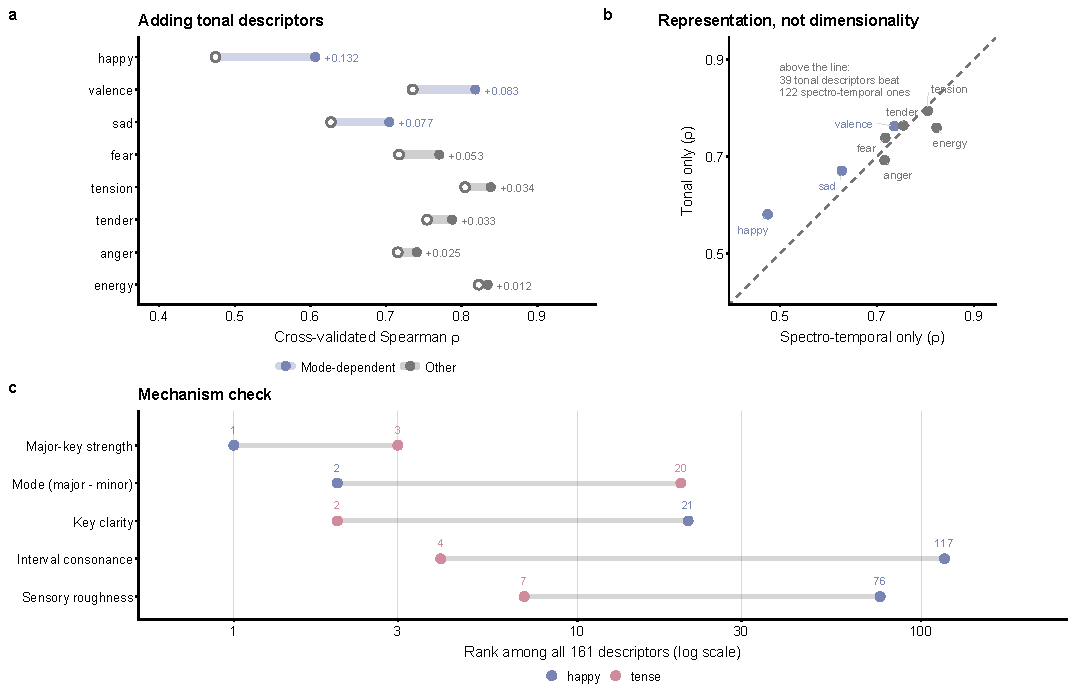
\includegraphics[width=\textwidth]{../reports/figures_r/Fig4_tonality.pdf}
\caption{A representation change recovers a specific deficit.
\textbf{(a)} Cross-validated Spearman $\rho$ for the eight affect axes of
Soundtracks ($n = 360$) with 122 spectro-temporal descriptors alone (open) and
with 39 tonal descriptors added (filled); axes ordered by gain. Blue marks the
three axes for which musical mode is theoretically decisive, a grouping fixed
before the comparison. \textbf{(b)} Tonal descriptors alone against
spectro-temporal alone: for happiness, 39 tonal descriptors ($\rho = 0.580$)
outperform 122 spectro-temporal ones (0.474), so the deficit was
representational rather than dimensional. \textbf{(c)} Mechanism check: rank of
five tonal descriptors among all 161 for happiness and for tension. Mode
carries perceived happiness; consonance and roughness carry perceived tension.
The preprint presented this as a falsification test of a two-kind framework;
that framing is withdrawn, since the framework is withdrawn and the test's
other half --- that more data does not close the happiness gap --- was never
measured.}
\label{fig:tonality}
\end{figure*}

Tonality is not the mechanism of the domain gap. Adding tonal descriptors
\emph{lowers} music-to-environmental transfer by 0.021 (18 paired comparisons,
$p = 0.038$ uncorrected), in the predicted direction but at a magnitude
accounting for roughly 4\% of the gap. Tonal descriptors contribute almost
nothing to arousal specifically ($+0.006$ within the music domain), and
arousal is the target on which the gap was measured.

\subsection{Boundary 2: cross-synthesis}
\label{sec:synthesis}

A deployed system never plays the corpus; it plays audio that has been
filtered, compressed, layered or generated. To ask whether the descriptors a
model relies on are ones that \emph{move} a prediction when altered, we edited
the audio: 80 source excerpts (40 music, 40 environmental) $\times$ three
interventions $\times$ four doses, with the model held fixed and only the
input changed (Fig.~\ref{fig:intervention}).

The perturbed models are binary random-forest classifiers of low- versus
high-arousal, one fitted on each domain; the modelled quantity is the
predicted probability of the low-arousal class, so a positive dose slope means
the edit made the excerpt read as \emph{calmer}. These are not the regression
models of Section~\ref{sec:corpus}, a distinction the preprint did not make.

Two of the three interventions passed their manipulation check --- the edit
moved the descriptor it was designed to move, monotonically across dose. Dose
response was tested per excerpt: a slope across the four doses, and a Wilcoxon
signed-rank test of those slopes against zero.

\subsubsection{The direction of the effect is not consistent across model and
material}

The preprint reported that spectral smoothing raised the low-arousal
probability in both domains (median slope $+0.015$, sign consistency 70\% for
the music model; $+0.074$, 71\% for the environmental model) and concluded
that "the sign of an acoustic manipulation crosses the boundary that the
predictions cannot, so what fails is calibration rather than the mapping".

Those statistics pool, for each model, the 40 excerpts of its own domain with
the 40 of the other. Disaggregated, the pattern does not support the
conclusion (Table~\ref{tab:intervention}). The music model shows the effect on
both kinds of material. The environmental model shows it strongly on
\emph{music} excerpts (median $+0.080$, 100\% sign consistency) and
\emph{not} on environmental excerpts --- the material it was fitted on and the
material the claim is about --- where the median slope is $-0.019$ in the
wrong direction at 57.5\% sign consistency and $p = 0.073$.

We therefore withdraw the claim. Three of the four model $\times$ material
cells move in the intended direction and one does not, and the one that does
not is the cell the mechanism claim needs most.

\begin{table}[!t]
\centering
\caption{Spectral smoothing, disaggregated by model and by the domain of the
material. Per-excerpt dose slopes on the predicted low-arousal probability;
positive means the edit made the excerpt read as calmer. The pooled rows are
the statistics the preprint reported.}
\label{tab:intervention}
\small
\setlength{\tabcolsep}{4pt}
\begin{tabular}{llccc}
\toprule
Model & Material & $n$ & \thd{Median}{slope} & \thd{Wilcoxon}{$p$} \\
\midrule
\multirow{3}{*}{Music}
 & pooled (as reported) & 80 & $+0.015$ & $3\times10^{-4}$ \\
 & music excerpts       & 40 & $+0.099$ & $2\times10^{-4}$ \\
 & environmental        & 40 & $+0.012$ & $7\times10^{-4}$ \\
\midrule
\multirow{3}{*}{Environmental}
 & pooled (as reported) & 80 & $+0.074$ & $<10^{-4}$ \\
 & music excerpts       & 40 & $+0.080$ & $<10^{-4}$ \\
 & \textbf{environmental} & 40 & $\mathbf{-0.019}$ & \textbf{0.073} \\
\bottomrule
\end{tabular}
\end{table}

A second defect affects how the sign-consistency statistic should be read. It
is defined as the fraction of excerpts whose slope matches the sign of the
observed median, so 50\% is its arithmetic floor rather than a chance level;
under the null its median is 0.54. Values near 50\% therefore indicate no
per-excerpt effect, and values of 57--60\% are close to that floor. Only the
cells at 70\% or above are meaningfully above it.

Independently of the data, the mechanism claim was incompatible with the
metric. Every transfer number in this paper is a Spearman rank correlation,
which is exactly invariant under any strictly monotonic recalibration of a
model's output. A purely calibrational deficit therefore \emph{cannot} move
$\rho$ at all, let alone from 0.591 to 0.115. Whatever fails at the domain
boundary changes the ranking, so it is not calibration in that sense.

\subsubsection{What the synthesis boundary does support}

Injecting transients moved the probability in the intended direction and
reached nominal significance in the pooled analysis but moved only 50\% and
59\% of excerpts consistently, at the statistic's floor; we report it as a
mean shift with no reliable per-excerpt effect. Envelope compression did not
achieve its intended descriptor change and is a failed manipulation rather
than a null result.

\begin{figure*}[!t]
\centering
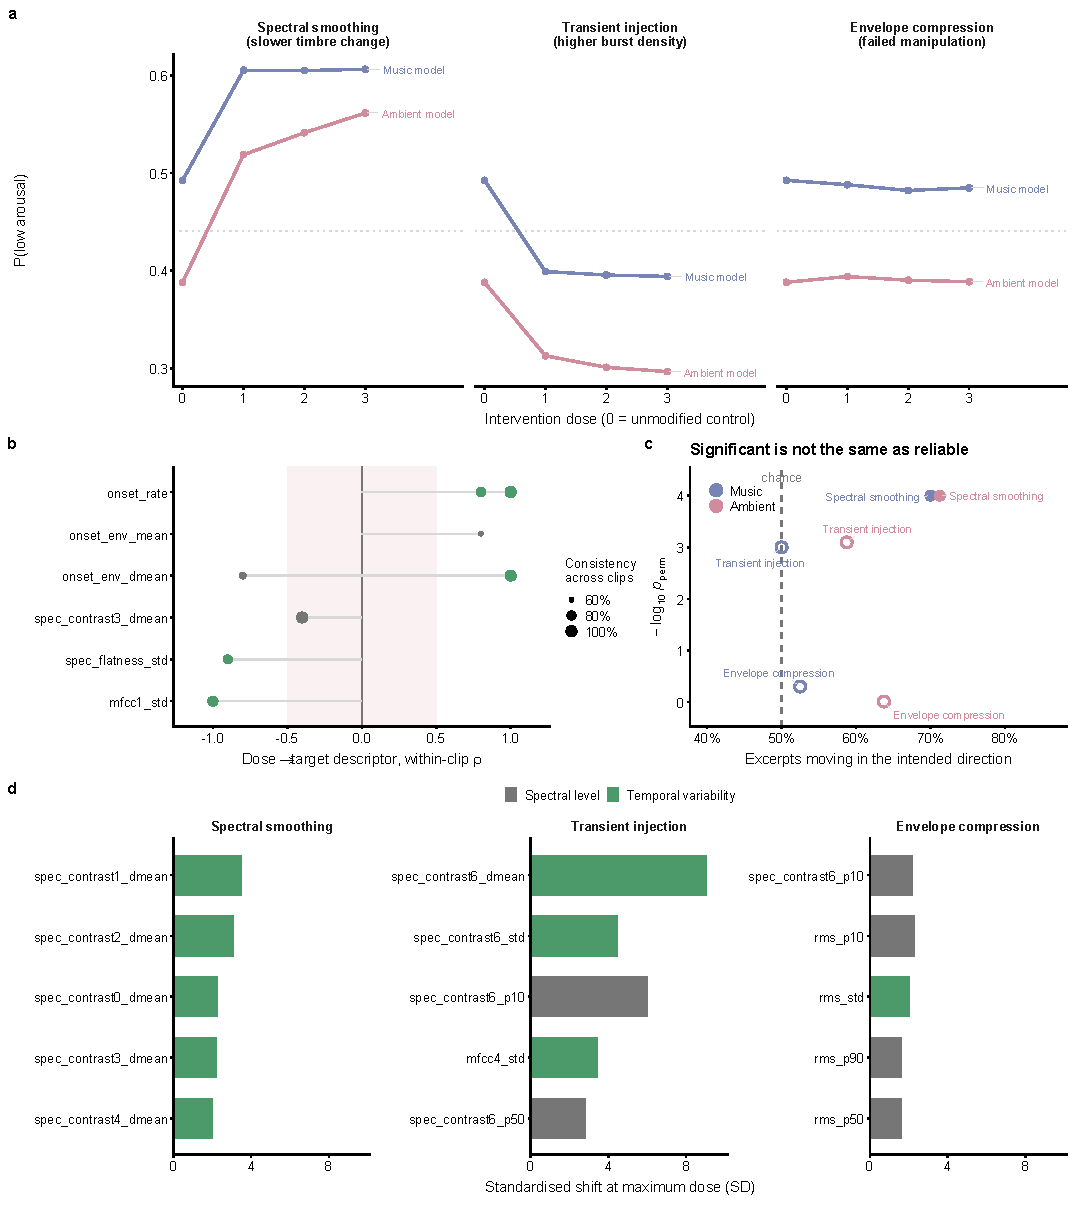
\includegraphics[width=\textwidth]{../reports/figures_r/Fig5_intervention.pdf}
\caption{An acoustic edit moves model output, reliably per excerpt for only
one of three interventions and only at the level of a descriptor dimension.
\textbf{(a)} Dose--response for three interventions on 80 excerpts at four
doses; curves are mean predicted probability of the low-arousal class, so a
rising curve means the edit made the excerpt read as calmer.
\textbf{(b)} Manipulation check, run before any dose--response was read.
Envelope compression fails it and is carried through as a failed manipulation
rather than as a null effect. \textbf{(c)} Specificity: the five descriptors
moved most by each intervention at maximum dose. No intervention moves its own
target descriptor most, which restricts claims to a descriptor
\emph{dimension}. \textbf{(d)} Significance against per-excerpt reliability.
Sign consistency is computed against the observed median's sign, so 50\% is
its arithmetic floor and not a chance level (null median 0.54). Panels
\textbf{(a)} and \textbf{(d)} pool each model's own-domain and other-domain
excerpts; Table~\ref{tab:intervention} disaggregates them, and that pooling
carried the preprint's withdrawn ``calibration, not sign'' claim. Every
quantity here is model output; no listener heard an edited excerpt.}
\label{fig:intervention}
\end{figure*}

A specificity diagnostic bounds what may be claimed
(Fig.~\ref{fig:intervention}c): no intervention moved a single descriptor in
isolation, each shifted a correlated family, and no intervention moved its
own target descriptor most. Transient injection moves
\texttt{spec\_contrast6\_dmean} by 9.0 standard deviations while moving
\texttt{onset\_rate} by 2.0, ranking its target twelfth. Claims are therefore
available at the level of a descriptor \emph{dimension} and not of any
individual descriptor.

Finally and most importantly, every statement in this section is about model
output. No listener heard any edited excerpt. Nothing here establishes that a
listener's affective response would move in the same direction, or in any
direction.

\subsection{Boundary 3: cross-response-channel}
\label{sec:channel}

This boundary is crossed by changing what counts as the response while the
sound and the listeners stay fixed. It is the boundary an application crosses
when it stops asking people how they feel and reads a sensor instead. It also
involves two different corpora and two different physiological modalities,
which the preprint fused under a single umbrella; we keep them separate.

\subsubsection{What was excluded before the question was asked}

Two analyses were removed on criteria unrelated to what they might have shown.
In ds002721 the documented mapping from stimulus trigger code to audio file
does not reproduce, and an attempt to recover it by matching emotion profiles
did not beat its permutation null ($p = 0.19$); acoustics-to-physiology is
therefore \emph{not testable} in that corpus and we do not test it
(Supplementary Section~S1). In BIRAFFE2 no participant of 94 passed both
electrodermal positive controls, so that pipeline is withdrawn (Supplementary
Section~S2) and supports nothing here.

\subsubsection{EEG: ratings carry more stimulus-specific structure than EEG
measures do}

Against the four passing controls, stimulus-level reliability was estimated
for eight self-report scales and 156 EEG measures on the same 31 listeners and
with the same estimator (Fig.~\ref{fig:channel}). Coherence is the strongest
EEG family (maximum intraclass correlation 0.092, 95\% CI [0.037, 0.142]) and
band power the weakest (0.040), against 0.221 [0.155, 0.281] for the
best-agreeing self-report scale.

\begin{figure*}[!t]
\centering
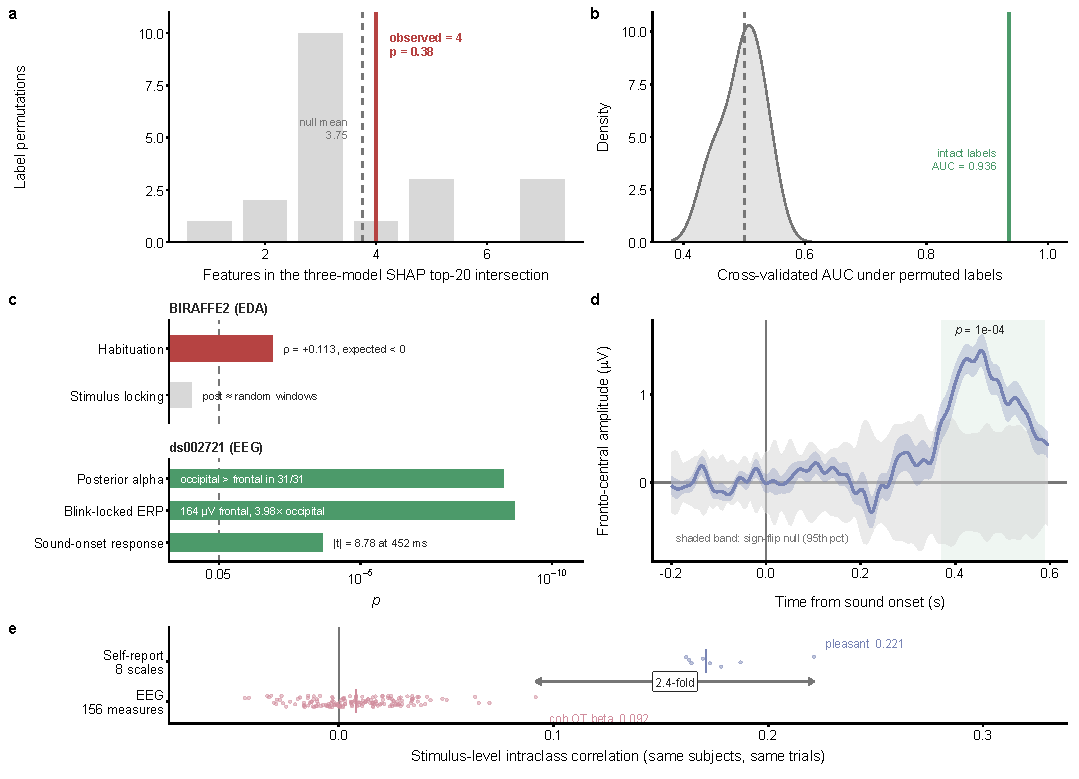
\includegraphics[width=\textwidth]{../reports/figures_r/Fig6_channel.pdf}
\caption{Reference distributions, positive controls, and the comparison they
license. \textbf{(a,\,b)} A cross-model attribution consensus against its
label-permutation reference: the observed overlap falls at the null mean
($p = 0.38$) while the intact labels reach an AUC of 0.936, so the statistic
cannot separate signal from noise and no claim is built on it.
\textbf{(c)} Positive controls for two physiological pipelines. BIRAFFE2 fails
both, and is withdrawn; ds002721 passes all. \textbf{(d)} Grand-average
fronto-central response to sound onset ($n = 31$); grey band, 95th percentile
of a subject-wise sign-flip null with max-statistic correction; peak
$|t| = 8.78$ at 452\,ms, $p = 0.0001$. \textbf{(e)} Stimulus-level intraclass
correlation for eight self-report scales and 156 EEG measures on the same
listeners. The EEG value is the maximum of 156 candidates and the self-report
value the maximum of 8, so their selection biases are unequal in the direction
that favours the EEG side; and the two sets rest on 1{,}240 and
1{,}080--1{,}121 trials respectively, not on identical trials as the preprint
stated. Reported as a bound, not an absence.}
\label{fig:channel}
\end{figure*}

Four qualifications are required, and the preprint stated only the first two.
The EEG value is the maximum of 156 measures and is biased upward for that
reason; referred to a null built the same way --- permuting stimulus labels,
recomputing all 156 correlations and taking the largest, 400 times --- it
carries $p = 0.02$, while Benjamini--Hochberg across the same 156 does not
pass it (smallest $q = 0.16$). It is close to the 0.10 this design resolves
with 80\% power, so the interval is consistent with values from near zero
upward. Third, the self-report value is also a maximum of a selection, but
over 8 candidates rather than 156, so the two point estimates carry
\emph{unequal} selection bias in the direction that favours the EEG side; the
comparison is conservative with respect to our conclusion but the asymmetry
should be stated. Fourth, the two sets are not computed on identical trials:
the EEG measures use 1{,}240 trials over 307 stimuli and the self-report
scales 1{,}080--1{,}121 trials over 285--298 stimuli. The preprint's claim of
"the same 1,240 trials" for both is incorrect.

What the data support is a comparison and not an absence: whatever
stimulus-specific structure these EEG measures carry is less than half of what
the listeners' own ratings carry on largely overlapping trials. This is a
statement about the component shared across listeners. It is not a claim that
the brain does not respond to sound --- the onset response in these same
recordings is large and highly reliable ($|t| = 8.78$ at 452\,ms,
$p = 0.0001$). What is weak is the \emph{differentiating} component.

A positive result exists in the literature on these same recordings and we
state its relation to ours precisely, because a reader could otherwise take
the two as contradictory. Daly et al.\ \cite{daly2015} report that
music-induced emotion can be predicted from brain activity \emph{combined
with} acoustic features, at a best correlation of $r = 0.234$
($p < 0.001$), with either feature type alone performing significantly worse.
We do not contradict that. It is a group-level, within-dataset prediction
result combining two modalities; ours is a stimulus-level reliability estimate
on EEG measures alone, asked in order to bound what a mapping from acoustics
could reach. The two are compatible: a combined model can predict an outcome
that an individual channel carries only weakly. We also note that the
acoustics half of their analysis requires the trigger-to-audio mapping we were
unable to reproduce (Supplementary Section~S1), which is why we do not attempt
the corresponding analysis here rather than reporting it as a failure.

\subsubsection{Electrodermal: no acoustic route exceeds its control, and no
ceiling can be quoted}

In PMEmo, three routes to the song-level electrodermal measures were compared.
Acoustic descriptors predict them at $\rho = 0.014$--0.070 with $p$ between
0.03 and 0.34; ratings predicted from acoustics reach $\rho = 0.091$--0.119;
and the listeners' own ratings reach $\rho = 0.117$ ($p = 0.004$, valence
against skin-conductance response rate). A random projection of the descriptor
space reaches the level of the two acoustic routes at its 95th percentile. The
defensible statement is therefore: \textbf{no acoustic route to these
electrodermal measures exceeds an uninformative control, and the listeners'
own ratings do, weakly.}

The preprint expressed all three as percentages of an attainable ceiling ---
31\%, 24.5\% and 21.3\% --- and argued that three routes stopping within a
third of the ceiling made it unlikely that the limit lay in the predictor.
Three things are wrong with that argument and we withdraw it in full.

First, the ceiling is not established. It was $\sqrt{r}$ of the measure's
stimulus-level reliability, and Section~\ref{sec:hazards} shows that
presentation position alone reproduces 114--249\% of that reliability. A
denominator that a position sham reproduces cannot bound a stimulus-driven
predictor.

Second, the percentages selected across denominators. The three figures use
two different electrodermal measures whose ceilings differ by 40\%, and the
largest percentage belongs to the measure with the \emph{lowest} reliability
and therefore the lowest ceiling --- not to the largest correlation. The
highest raw correlation (0.135, valence against phasic mean) yields the
\emph{smaller} percentage.

Third, the preprint asserted that the three routes' confidence intervals
overlap. No confidence intervals were computed for the acoustic routes. The
one interval that does exist, for the rating route, contains the
random-projection control.

Finally, the three routes are not independent evidence: route 2 is derived
from route 1 and route 3 is the source of route 2. Three nested routes failing
alike is weaker than three independent ones, which the preprint did not say.

What remains is a clean negative about the routes tested, on a target whose
own stimulus-level reliability this corpus cannot establish. We do not claim
that no quantity of target-side data would recover this gap, and we did not
measure a target-side learning curve on a physiological outcome. That
experiment is the single most informative one this work does not contain.

\subsubsection{The individual-level analysis is a design problem, not a null}

Because the intended application is per-person, the same question was asked
within listeners on the EEG corpus, with the null drawn from each listener's
own label permutations. Of 248 listener $\times$ scale tests, 9 reached
$p < 0.05$ against a chance expectation of 12.4 (binomial $p = 0.88$), and
none survived correction (Supplementary Fig.~S6).

Independent-component removal of ocular artefacts acts here as a sensitivity
manipulation check rather than as cleaning: it increased detection of the
known effect (individual-level control: 26 $\rightarrow$ 29 listeners passing,
$\rho = 0.401 \rightarrow 0.573$) while further reducing the effect of
interest (13 $\rightarrow$ 9 nominal detections). A pipeline made measurably
more sensitive did not reveal the association, which excludes insufficient
signal-to-noise.

It does not exclude insufficient observations. With the roughly 30 rated
trials each listener contributed, the design simulation below gives 10\% power
for a within-person association of $r = 0.40$ and 6\% for $r = 0.20$. The
individual-level analysis is therefore \textbf{uninformative} about
within-person associations below approximately $r = 0.5$, and we draw no
conclusion from it. The between-listener result does not share this
limitation, because it pools 31 listeners at the level of the stimulus.

\subsection{Boundary 4: cross-individual}
\label{sec:individual}

\subsubsection{How many observations per person a design needs}

Synthetic within-person associations of known strength were injected into data
generated from the empirical feature covariance of the EEG corpus
(Ledoit--Wolf shrinkage \cite{ledoit2004}) and recovered with the identical
pipeline, criterion and permutation test (Fig.~\ref{fig:design}b). The
requirement is steep: 314 observations per person for $r = 0.40$, 564 for
$r = 0.30$, 1{,}364 for $r = 0.20$ and 4{,}888 for $r = 0.10$, against the
$\sim$30 this corpus supplies (Table~\ref{tab:power}).

Because that rests on an assumed covariance structure, we measured the same
curve directly in ds003690, which supplies $\sim$240 auditory events per
person with simultaneous EEG, electrocardiogram and pupillometry and carries
an effect that is certainly present. Establishing it at the group level first
is what makes the individual-level result interpretable: at $p = 0.0002$ for
all three channels, an individual in whom it is not detected is one in whom
the measurement failed, not one in whom the effect is absent. The cardiac
component reproduces the anticipatory deceleration of $-0.83$\,bpm those
authors originally reported in this cohort \cite{ribeiro2019cardiac}.

At the full 240 observations the evoked response is recovered in 72 of 75
listeners from EEG, 62 of 73 from pupil diameter and 47 of 75 from heart rate.
At 30 observations --- what a laboratory session supplies --- the same effect
is recovered in 53\%, 39\% and 23\% of individuals, while the false-positive
rate stays nominal across the whole range (0.03--0.07)
(Fig.~\ref{fig:design}a). An effect plainly visible in the group average
($-5.6\,\uV$ at the N1) is a coin toss within a single person at the
observation count these paradigms provide.

\begin{figure*}[!t]
\centering
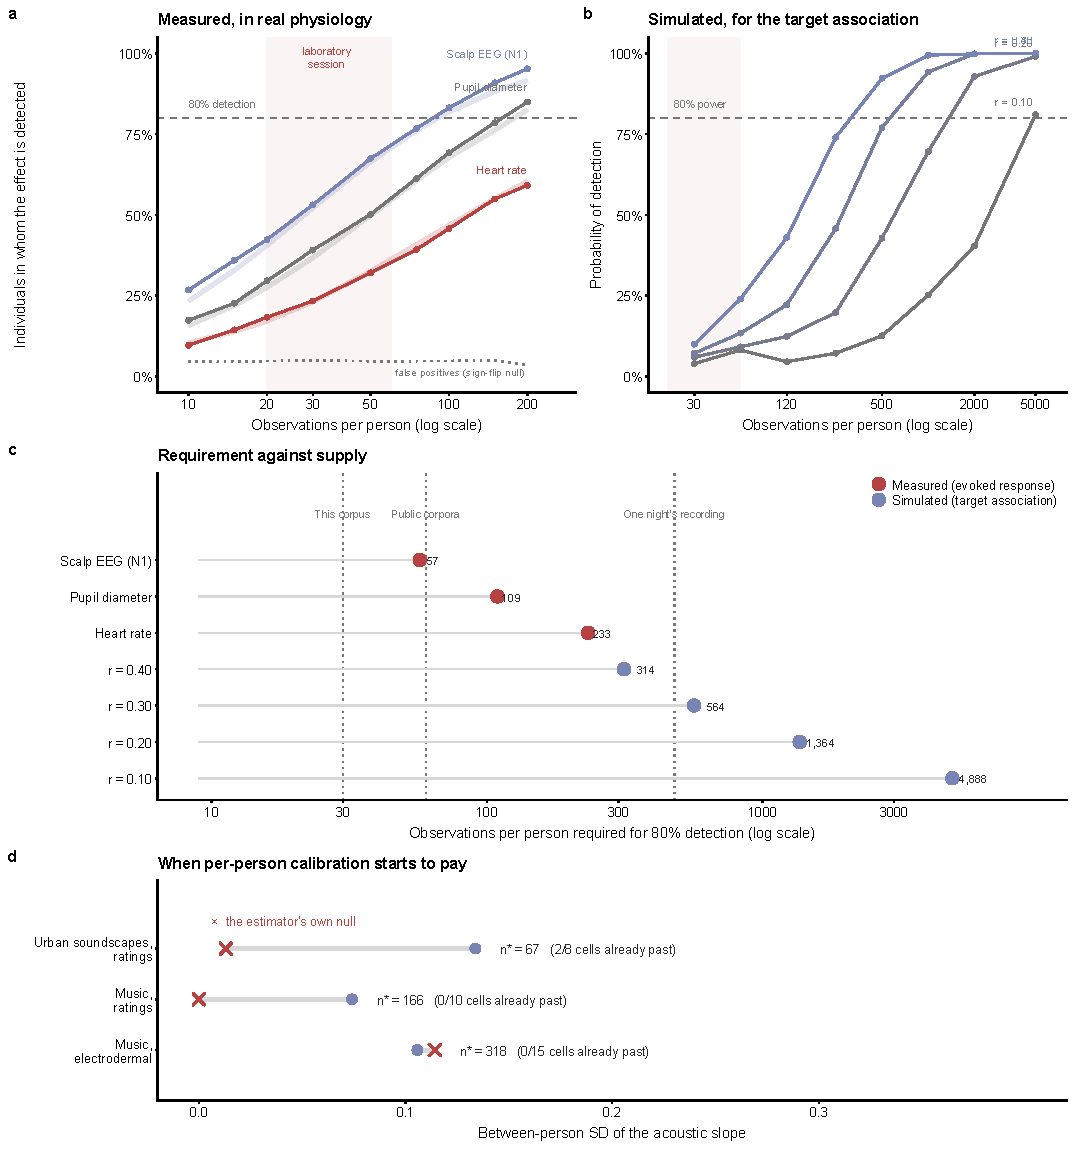
\includegraphics[width=\textwidth]{../reports/figures_r/Fig7_design.pdf}
\caption{The individual-level question is a design problem rather than a null
result. \textbf{(a)} Detection measured in real physiology: in 75 listeners
with $\sim$240 auditory events each, the proportion in whom the evoked
response is detected when only $n$ of that listener's observations are used (40
resamples per point), with each channel's analytic power curve overlaid. The
dotted line is the false-positive rate from sign-randomised differences and
stays nominal (0.03--0.07) throughout, so the rise is detection.
\textbf{(b)} Simulated power against observations per person for four true
association strengths. \textbf{(c)} Observations per person for 80\%
detection, measured and simulated, against three supply levels.
\textbf{(d)} Between-person slope spread and its per-cell
parametric-bootstrap null in three settings; the null is plotted rather than
subtracted because the estimator returns 0.11 at 18 observations per person
when the true value is zero. Panel \textbf{(d)} is a different quantity from
\textbf{(a)}--\textbf{(c)}, and its three settings differ in corpus,
descriptor set and outcome axis together, so they are not compared against one
another. Extended description in the Supplementary Information.}
\label{fig:design}
\end{figure*}

Three features bear on how the simulated requirement should be read. It
validates the extrapolation: predicting detection at $n$ from an effect size
estimated on a disjoint half of the same person's trials matches the observed
rate to within 0.03 on average. The requirement is channel-specific in the
direction that matters for applied work --- heart rate, the signal a consumer
device records, needs roughly four times as many observations as scalp EEG
(233 against 57). And it is not worse in older listeners; the evoked response
is larger in the older group, so fewer observations are needed (48 against 69
for EEG). Both kinds of estimate are lower bounds: the simulation assumes
multivariate normality, linearity and within-person stationarity, each of
which favours detection, and the measurement uses a deliberately plain
pipeline.

\begin{table}[!t]
\centering
\caption{Observations per person required for 80\% power, and the power
available at the $\sim$30 rated trials the EEG corpus provides. Simulated rows
use injected associations of known strength; measured rows use the auditory
evoked response in an independent corpus of 75 listeners.}
\label{tab:power}
\small
\begin{tabular}{llcc}
\toprule
& Effect & \thd{Obs.\ for}{80\% power} & \thd{Power at}{$n = 30$} \\
\midrule
\multirow{4}{*}{Simulated}
 & $r = 0.40$  & 314        & 0.10 \\
 & $r = 0.30$  & 564        & 0.07 \\
 & $r = 0.20$  & $1{,}364$  & 0.06 \\
 & $r = 0.10$  & $4{,}888$  & 0.04 \\
\midrule
\multirow{3}{*}{Measured}
 & Scalp EEG (N1)  & 57  & 0.53 \\
 & Pupil diameter  & 109 & 0.39 \\
 & Heart rate      & 233 & 0.23 \\
\bottomrule
\end{tabular}
\end{table}

One further result from that corpus bears on the choice of channel. In its
passive block, where the same tones are presented with no task and no
response, the cortical response is undiminished ($-5.7\,\uV$, $p = 0.0002$)
but neither the cardiac nor the pupillary response is detectable
($p = 0.30$ and $p = 0.99$). This is not a power failure: had the effect been
the size it is in the active blocks, the group test would have detected it
with probability 1.00. The scope of the observation is narrow --- 250\,ms
tones, awake listeners, 30 passive trials each --- and it does not transfer to
music heard over minutes. It does mean that for a passively listening user
monitored through heart rate alone, the question of how many observations are
needed may be preceded by the question of whether there is a response to
count.

\subsubsection{Between-person slope heterogeneity, and what it does not
establish}

The question an application faces is when fitting a listener their own slope
beats giving them the population slope. Table~\ref{tab:individual} reports two
answers, and they disagree.

The variance model places break-even at 67 observations per person in urban
soundscape ratings, 166 in music ratings, and --- over the minority of
electrodermal cells in which it is finite at all --- 318. Between-person
spread exceeds its own per-cell null in 8 of 8 soundscape cells, 10 of 10
music-rating cells, and only 4 of 15 electrodermal cells.

Three properties of the electrodermal row must be stated because the preprint
reported its $n^{*}$ as though it were comparable to the other two. Ten of the
fifteen cells have a corrected spread of exactly zero, so $n^{*}$ for them is
infinite: no budget buys a quantity that may be zero. The reported 318 is the
median over the five cells where $n^{*}$ is finite, a subset the preprint did
not disclose, and one of those five does not exceed its own null. The median
over all fifteen cells is infinite, and the median over the four cells that do
exceed their null is 264. We give all three and interpret none of them as a
price.

\begin{table*}[!t]
\centering
\caption{Between-person slope heterogeneity and break-even, with the direct
out-of-sample test alongside. $\tau$ is the between-person standard deviation
of the acoustic slope after subtraction of a per-cell parametric-bootstrap
null. $n^{*}$ is the model-implied break-even. The final column is the
measured out-of-sample gain from fitting each listener their own slope instead
of the population slope, at the observation count the corpus supplies.
Positive would mean personalisation helps.}
\label{tab:individual}
\small
\setlength{\tabcolsep}{3.5pt}
\begin{tabular}{lccccc}
\toprule
Setting & \thd{Obs.\ per}{person} & \thd{Cells above}{own null}
        & \thd{Median}{$\tau$} & \thd{Median}{$n^{*}$}
        & \thd{Out-of-sample}{gain} \\
\midrule
Soundscape ratings  & 42 & 8/8   & 0.133 & 67  & not measured \\
Music ratings       & 44 & 10/10 & 0.074 & 166 & $-0.054$ to $-0.020$ \\
Music electrodermal & 18 & 4/15  & 0.000 & $\infty$\,\textsuperscript{a} & $-0.109$ to $-0.072$ \\
\bottomrule
\multicolumn{6}{l}{\footnotesize\textsuperscript{a} 318 over the 5 cells with
finite $n^{*}$; 264 over the 4 above their own null.}
\end{tabular}
\end{table*}

\subsubsection{The direct test returns a negative gain at every budget
available}

The repository behind this paper already contained the out-of-sample test the
break-even framing needs, and the preprint did not report it. We report it
here because it is the more decisive evidence and it points the other way.

Fitting each listener their own slope and evaluating out of sample against the
population slope returns a \textbf{negative} gain in 15 of 15 electrodermal
cells ($-0.109$ to $-0.072$ at 18 observations per person) and in every one of
10 music-rating cells at 18, 30 and 50 observations per person. The gain rises
monotonically towards zero with budget: $-0.125$ to $-0.052$ at $n = 18$,
$-0.054$ to $-0.020$ at $n = 30$, $-0.028$ to $-0.002$ at $n = 50$, and at
$n = 100$ four of ten cells turn positive with the best at $p = 0.054$.

That trajectory is consistent with the variance model's break-even of 166 for
this setting, and to that extent it validates the extrapolation's direction.
It also settles the applied question in the opposite direction from the
preprint's reading: \textbf{at every observation count these corpora supply,
per-person calibration measurably loses to the population model.}

No out-of-sample test of this kind exists for the soundscape corpus, which is
the setting with the lowest $n^{*}$ and the only one where the model implies
break-even has been reached. The two cells said to have crossed break-even are
both on the eventfulness axis, and the manipulation check for that axis does
not pass in that corpus --- the sound-to-masker ratio manipulation moves
pleasantness ($p = 4 \times 10^{-6}$) but not eventfulness ($p = 0.38$). The
single positive individualisation result in this paper therefore sits on the
axis with no passing positive control and with no out-of-sample confirmation.
The defensible reading is that per-person calibration in the
product-adjacent domain is \emph{worth testing} at a scale existing corpora
reach, and that it has not been shown to pay anywhere.

For the same reason we do not compare the three settings against one another.
Corpus, descriptor set and outcome axis vary together: the soundscape cells
use ISO-532 psychoacoustic descriptors against ISO soundscape axes, the music
cells use spectro-temporal and tonal descriptors against valence and arousal,
and the electrodermal cells use those same descriptors against electrodermal
measures. The preprint concluded from the spread that "choosing the wrong
corpus is as expensive as choosing the wrong channel"; with three covarying
factors and three settings, that conclusion is not available.

% =====================================================================
\section{Discussion}

\subsection{What the evidence supports}

Reported as a ledger rather than a verdict, the four boundaries divide by
evidence state rather than by kind of failure.

\emph{Improvement observed.} On the corpus boundary, both the same-domain and
the cross-domain gap are substantially recoverable. One hundred target-side
labels recover about half of either gap and 200 recover two-thirds to
three-quarters; label-free correlation alignment recovers a quarter of the
cross-domain gap, and a valid sham establishes that this gain is
target-specific. A targeted representation change recovers a specific
deficit --- tonal descriptors for perceived happiness --- that the
spectro-temporal set does not reach.

\emph{No improvement observed under the routes tested.} Four pretrained
representations did not recover the cross-domain gap; on a leak-free test set
the best of them improves on 122 hand-specified descriptors by 0.034 in rank
correlation, against a gap of 0.49. No acoustic route to
song-level electrodermal measures exceeded a random-projection control. No
within-person EEG--rating association was detected, and no per-person
calibration gain was observed out of sample at any available budget. In each
case the statement bounds the routes we ran, and in none of them do we claim
that the information required is absent from the input.

\emph{Insufficient evidence.} Whether the music/environmental gap is a
property of the sound domain or of Emo-Soundscapes specifically cannot be
decided with one environmental corpus, particularly as that corpus also
differs in annotation method. Whether CLAP's advantage reflects pretraining
overlap or greater strength on environmental sound cannot be separated.
Whether the electrodermal negative reflects the channel, the predictor or the
target's measurement cannot be decided in a corpus where presentation position
reproduces the target's reliability. And whether per-person calibration pays
at 67 observations per person is untested in the one setting where the model
says it should.

The single most useful practical consequence is about reporting convention. A
zero-shot cross-corpus number is an upper bound on the generalisation problem,
not an estimate of it. On the cross-domain boundary, where the unadapted loss
is 75\% of the target's own within-corpus reference, a hundred target-side
labels recover 57\% of the gap that loss opens and a label-free second-moment
alignment recovers 25\% of it with no labels at all. We quote those recovery
fractions rather than composing them with the loss into a residual, because the
loss is a median over six algorithms while the recovery fractions are measured
on ridge --- multiplying the two would be exactly the mismatched-denominator
error this paper spends a section correcting. A field that reports the first
number and not the second systematically overstates how badly its models
generalise --- and, by the same token, a field that reports an alignment gain
without a valid sham overstates how well adaptation works.

\subsection{Two hazards for anyone reusing these corpora}

Both are properties of widely used public corpora rather than of our analysis,
and both are actionable.

In Emo-Soundscapes, grouped cross-validation on the supplied group identifiers
gives no protection against near-duplicate mixture clips spanning folds. The
correct grouping is recoverable from the filenames, which encode the
constituents; because every mixture shares a constituent with some other
mixture, a connected-components grouping collapses all 613 into one group, so
the practical options are to evaluate on the 600 originals or to hold the
mixtures out as a block. On our data the difference is 0.10 in the
within-corpus reference and a factor of three in cross-domain transfer.

In PMEmo, any analysis that treats the song-level electrodermal measures as
stimulus-driven --- including any that uses their reliability as a ceiling ---
needs a presentation-position control first.

\subsection{Threats to validity}
\label{sec:threats}

\emph{One environmental corpus.} Every cross-domain cell in this paper
involves Emo-Soundscapes, so "crossing a domain boundary" and "transferring to
this corpus" are the same operation. The corpus differs from the three music
corpora in sound domain, in annotation method (pairwise comparison versus
direct rating), in clip length and in provenance. We report the result as
measured and do not attribute it to the domain alone. Resolving this needs a
second environmental affective corpus, which we were unable to obtain in a
form permitting this analysis.

\emph{Units of replication.} The 36 same-domain and 36 cross-domain transfer
values are 6 ordered corpus pairs each evaluated with 6 algorithms. The
algorithms are not independent replications; the corpus pairs are the units,
and there are six of each kind. Dispersion statistics over 36 values should be
read accordingly.

\emph{Shared material between corpora.} The stimuli of the EEG corpus
ds002721 are excerpts from the Soundtracks set used as our fourth music
corpus. Results involving both are not independent.

\emph{Selection and multiplicity.} The 84.4\% within-corpus figure is the best
of six algorithms; the EEG intraclass correlation is the maximum of 156
measures and the self-report value the maximum of 8, an asymmetry that
favours the EEG side. No multiplicity control is applied across the 33
per-person calibration cells. The per-cell nulls for those cells rest on 60
bootstrap replicates, so Monte-Carlo error on the threshold is of the same
order as the margin by which the marginal cells clear it, and the slopes are
estimated in two stages where a cross-classified hierarchical model would
propagate the first stage's uncertainty into the second.

\emph{Construct scope.} This paper moves between model outputs,
group-averaged perceived-emotion ratings, individual self-report, EEG
measures, electrodermal measures, heart rate and pupil diameter. These are not
interchangeable and a result on one does not stand in for another. In
particular, perceived arousal in a rating corpus is not sleep onset, sleep
continuity or any clinical endpoint; no analysis here relates a naturalistic
soundscape to a peripheral physiological measure; and nothing in this work
bears on the efficacy of audio for sleep. Cardiac and pupillary signals enter
only through the design-requirement measurement, where the stimulus is a
250\,ms tone presented to awake listeners performing a task.

\emph{No prior specification.} As stated in the Methods, we can produce no
traceable artifact predating the analyses for any criterion, and nothing here
is preregistered.

\subsection{What would settle the open questions}

Three experiments, in order of how much they would change.

A target-side learning curve on a physiological outcome. Everything we can say
about that boundary concerns the routes we tried; only a budget curve
distinguishes a gap that observations close from one they do not, and none
exists.

A second environmental affective corpus, annotated by the same method as the
music corpora, outside the pretraining data of the representations under test.
That single addition separates domain from dataset, annotation method from
sound, and pretraining overlap from representational strength.

Within-person longitudinal data with varied stimuli. The requirement measured
here is 57 to 233 observations per person depending on channel, and the corpora
available supply 18 to 44. The shortfall is in duration and repetition, not in
participants: recruiting more people does not provide observations within a
person. Observation count and stimulus richness also trade against each other
inside a fixed session --- the corpus that supplies 240 events per person does
so with four pure tones --- and it is the combination that no session-length
design provides. A search of OpenNeuro (1{,}833 datasets) and PhysioNet (426)
returned no corpus pairing repeated controlled auditory stimulation with a
state readout at the required density, and the standard affective-physiology
corpora distributed elsewhere supply 8 to 40 stimuli per participant. That
claim is bounded by the search rather than absolute.

% =====================================================================
\section{Conclusion}

Across four boundaries, the generalisation losses an affective audio model
suffers are large when measured zero-shot and substantially smaller when a
modest adaptation budget is quoted alongside them. On the cross-domain corpus
boundary the unadapted loss is three-quarters of the target's own within-corpus
reference, and of the gap that opens, a hundred target labels recover 57\% and
a label-free second-moment alignment recovers a quarter with no labels at all
--- a gain a sham control supports as target-specific on the three pairs where
that control is valid. On the response-channel and
individual-listener boundaries we found no route that recovered the gap, and
we report that as a bound on the routes tested rather than as a property of
the input, because the experiments that would distinguish the two --- a
target-side budget curve on a physiological outcome, and an out-of-sample
personalisation test in the product-adjacent corpus --- were not available to
us. Two of the corpora we used carry structural hazards that inflate
within-corpus performance and distort any ceiling computed from them, and both
are recoverable from the distributed metadata. We would rather report a
measured price list with three acknowledged gaps in it than a framework that
the same measurements contradict.

% =====================================================================
\section{Declarations}
\label{sec:declarations}

\emph{Ethics.} This work is a secondary analysis of de-identified data
released for public reuse. No new data were collected from human participants
and no attempt was made to re-identify any individual. Approval provenance
differs across the nine corpora and is stated per corpus in Supplementary
Table~S13: where the source publication reports an approving body and protocol
identifier we cite it; where it does not, we state that no approval statement
is available in the source rather than implying one exists.

\emph{Competing interests.} The authors are engaged in the development of a
commercial sleep-audio product. Nothing in this paper bears on the efficacy of
audio for sleep. Four of the corpora used here could not enter such a product
in any case, for two different reasons: ESC-50 and ARAUS carry non-commercial
terms, and the audio of PMEmo and of Soundtracks carries no redistribution
right --- the latter because the Soundtracks deposit's own CC~BY~4.0 licence
does not convey rights in the commercially released recordings it excerpts. One
of the pretrained representations, MERT, is likewise non-commercial.

% Section numbers are \ref rather than literals so they cannot drift if the
% document is reordered. They resolve to III-D, IV-B and IV-D, which is how the
% authors wrote them.
\emph{Use of generative AI.} Claude (Anthropic) was used under author direction
to generate and revise analysis code, assist with pre-submission consistency
checks, execute the reanalyses reported in
Sections~\ref{sec:hazards}, \ref{sec:corpus}, and \ref{sec:synthesis}, and
draft and revise text throughout the manuscript and supplementary material.
Numerical analyses and figures were produced by executing the analysis and
plotting scripts described in the repository. The authors reviewed the
AI-assisted text and code, checked the reported results against the analysis
outputs, and verified the references. Generative AI was not used to fabricate
participant records or empirical observations; simulations and audio
transformations are described in the Methods. The authors take full
responsibility for the methods, results, interpretations, and final manuscript.

\emph{Data availability.} All analyses use publicly available data. Accession
identifiers, access dates and licence terms are listed in Supplementary
Table~S14. No new data were generated. Derived tables underlying every figure
panel are provided as supplementary source data and are archived with the code
at \url{https://doi.org/10.5281/zenodo.23044439}.

\emph{Code availability.} Analysis code, run records and figure-generation
scripts are at \url{https://github.com/AuraJZ/affective-audio-boundaries} and
are archived at \url{https://doi.org/10.5281/zenodo.23044439}, which resolves
to the current version. Each reported value has a run record identifying the
script, the random seed
and the parameters. The limits of that record are material and are stated
rather than glossed: all run records were written from a working tree with
uncommitted changes and the repository head is older than most of the
analyses, so the recorded commit identifies a starting point and not the state
that produced the number; input hashes are present for 38 of 199 records and
output hashes for none; there is no automated test suite. The analyses are
reproducible from the scripts and the public corpora at the parameters
recorded, and are not reproducible bit-for-bit from a pinned commit. We do not
claim the stronger guarantee.

\emph{Author contributions.} \textbf{J.Z.}: conceptualisation; methodology;
software; validation; formal analysis; investigation; data curation;
visualisation; writing --- original draft; writing --- review and editing.
\textbf{X.Y.}: conceptualisation; resources; validation; writing --- review
and editing; project administration.

\section*{Acknowledgements}

We thank the investigators who released the datasets analysed here. This work
would not have been possible without their decision to make the recordings,
annotations and event files public.

\bibliography{../references/references}

\end{document}
